\chapter{FCS 的群体感受扩展：流体群体智能、SFPU 与跨尺度具身协同}

\begin{chapteroverviewbox}
前一章已经建立了 AgentOS 面向现实世界的二元接口：SGC（Semantic Graph Coordinate Space）负责描述“现实中有什么、它们在哪里以及彼此具有怎样的语义关系”，FCS（Feeling Coordinate/Field System）负责描述“这些现实状态正在如何作用于本体”。在此基础上，本章进一步研究一个自然但具有重要架构意义的问题：当一个独立 Agent 不再只通过视觉、触觉、本体感觉、能源状态等普通 Body Driver 感知现实，而开始成为一个大规模机器人群体的一部分时，群体宏观结构应当通过什么接口进入本地 AgentOS？

本章给出的答案是：\textbf{群体协调不应该首先表现为一个外部中央系统对本地 AgentOS 的强制命令，而应首先表现为一种新的身体感受。} 为此，我们引入 SFPU（Swarm Field Processing Unit）。在软件架构意义上，单个 SFPU 被严格定义为 AgentOS Body Driver 体系中的一种特殊群体场驱动器；多个 SFPU 通过 Field Plane 互联后共同形成分布式群体场网络；独立于本地 AgentOS 的 SwarmOS 通过 Potential Plane 向 SFPU 提供群体任务势能和目标嵌入；SFPU 再通过局部场重构与势能微分产生物理梯度和语义梯度，并经 Gradient Plane 映射为 FCS 中的一种特殊“群体梯度感受面”。

因此，本章并不试图把群体智能并入单体 AgentOS 内核，而是建立一个严格的跨尺度耦合关系：
\[
\boxed{
SwarmOS
\rightarrow
Potential
\rightarrow
SFPU
\rightarrow
Gradient\ Sensation
\rightarrow
FCS
\rightarrow
AgentOS
\rightarrow
Body
\rightarrow
Collective\ Field
}
\]
其中，群体层提供宏观结构约束，个体层保留本体认知、边界与最终行动决策权。由此，FCS 不再只是“身体内部感受场”，而获得了一种更一般的含义：\textbf{任何能够以本体为参照表达“现实结构对我产生怎样方向性影响”的结构化场，都可以作为一种 FCS 感受面接入 AgentOS。}
\end{chapteroverviewbox}

\begin{figure}[htbp]
\centering
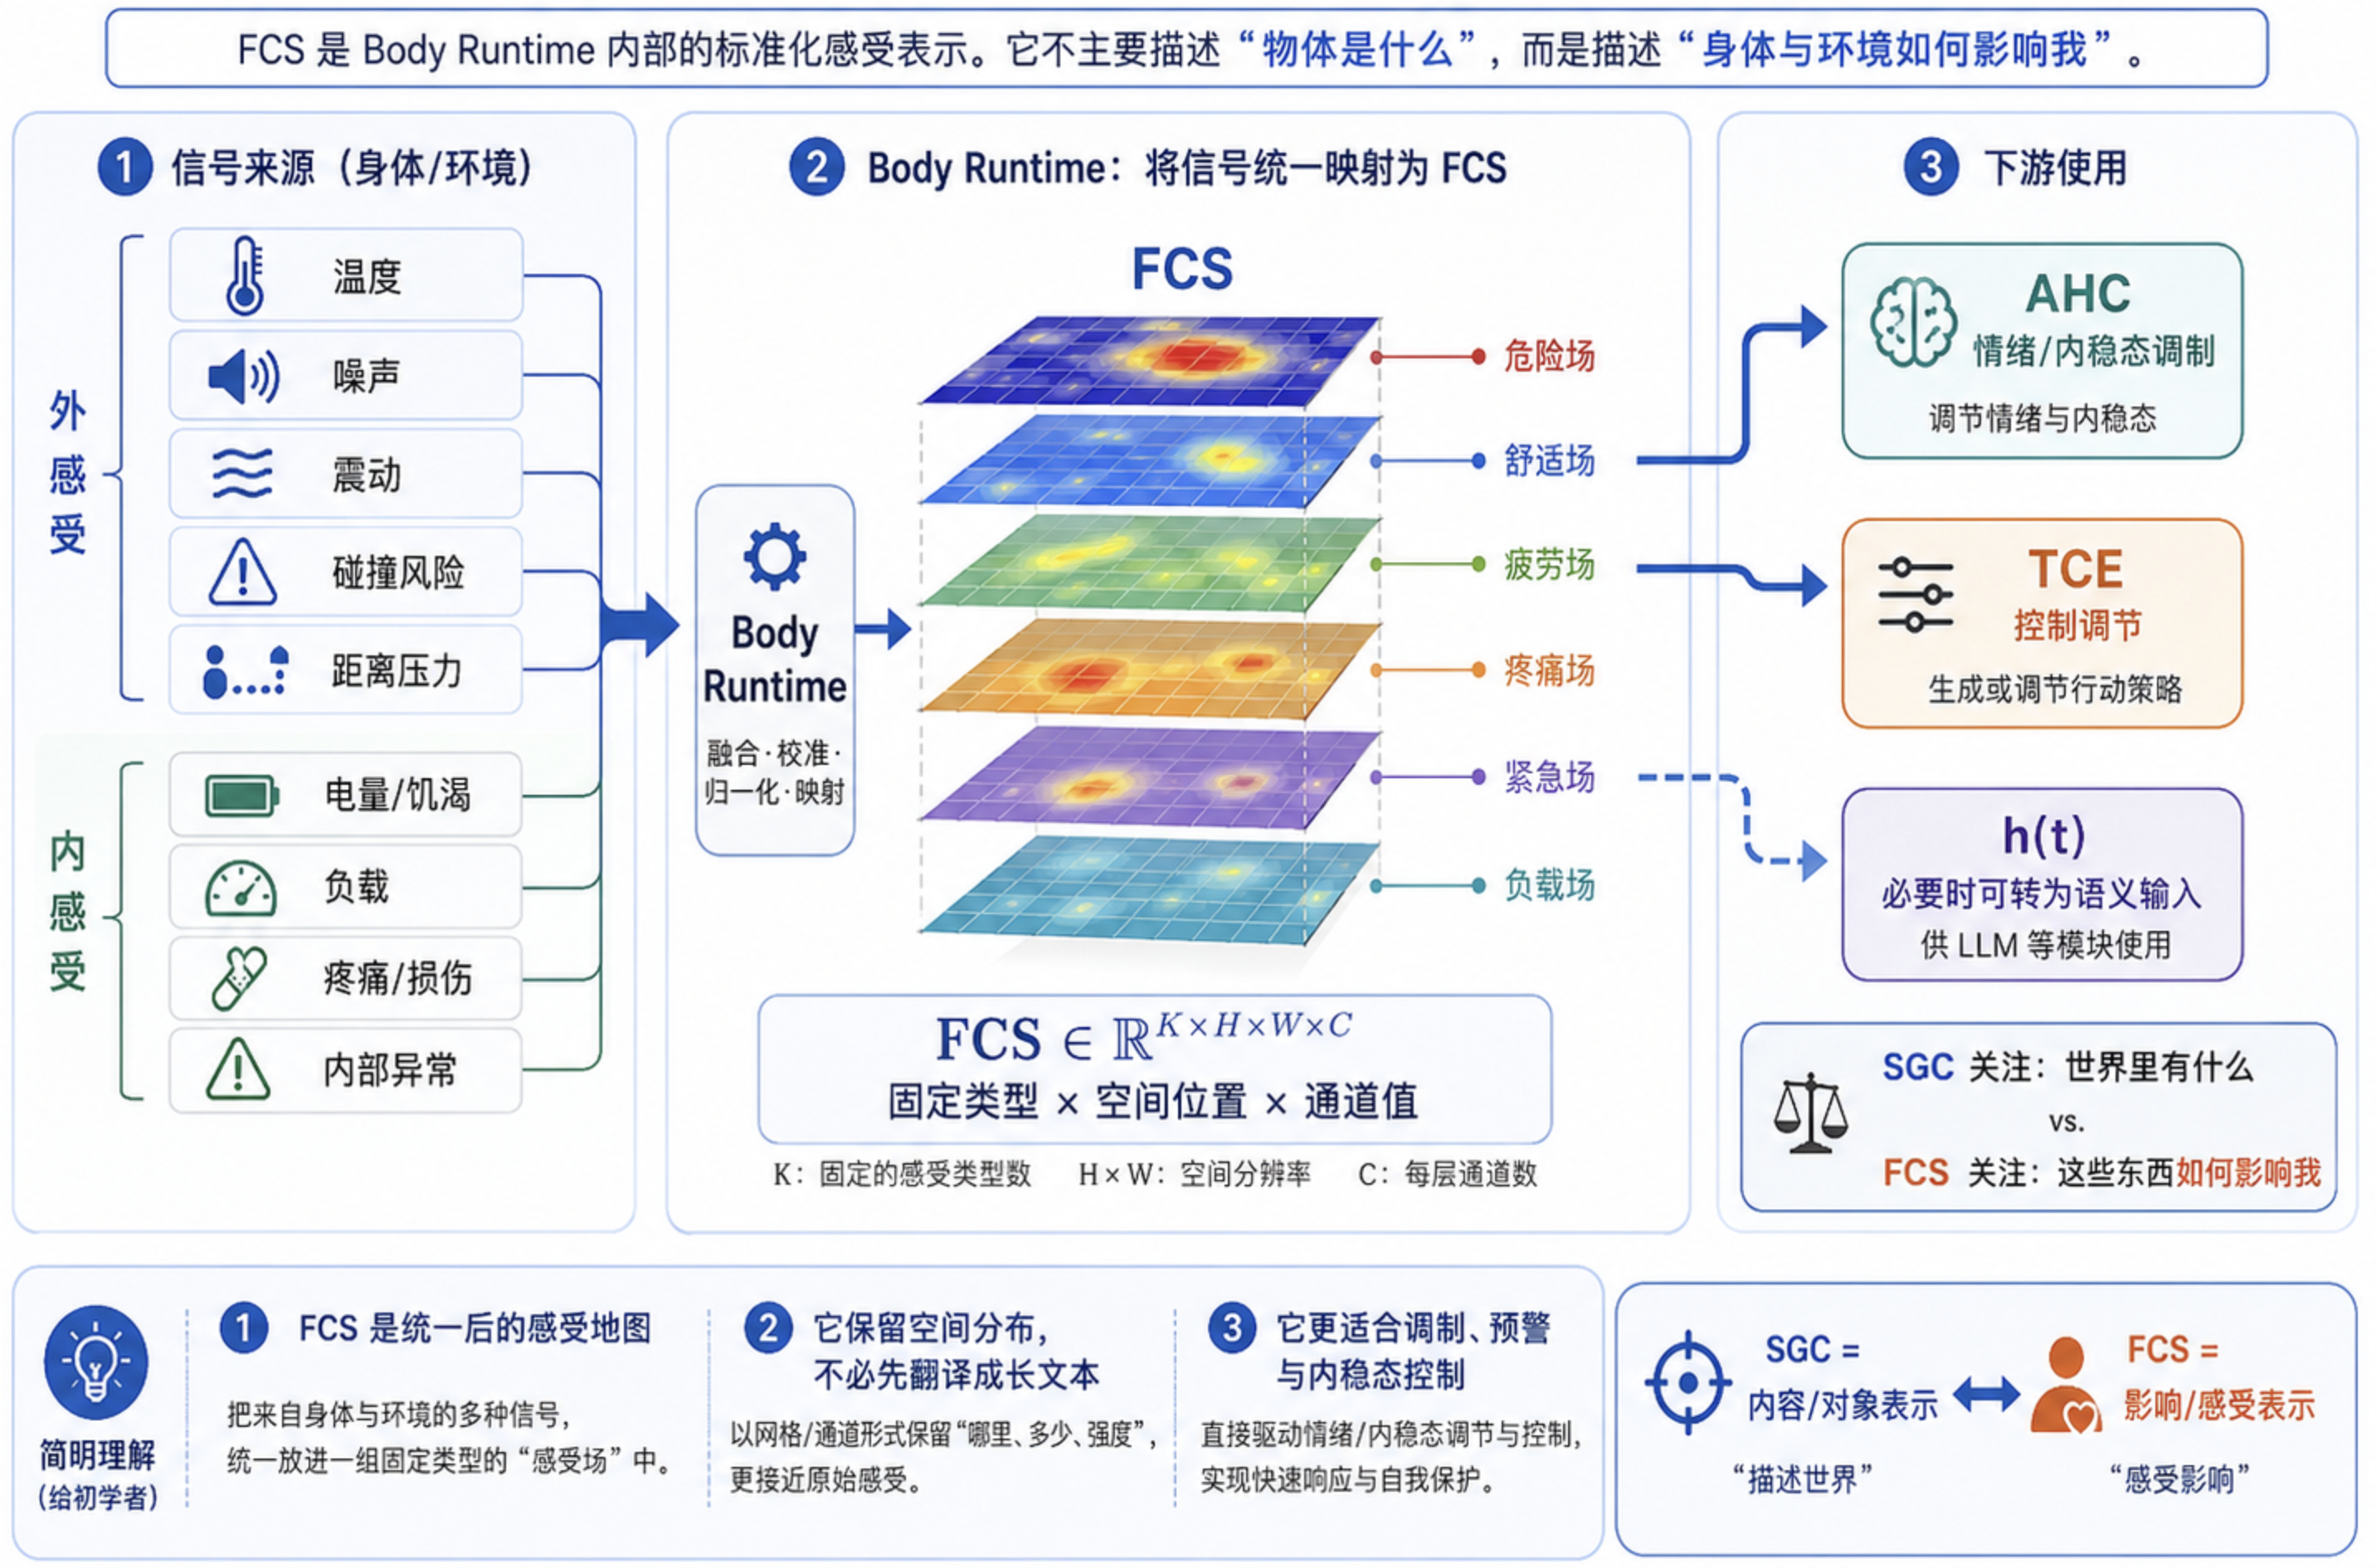
\includegraphics[width=.9\textwidth,height=.38\textheight,keepaspectratio]{images/FCS-Repect.png}
\caption{FCS的多通道实现示意图}
\end{figure}

\section{从 SGC--FCS 二元现实接口到群体感受面}

在前一章中，我们已经把 AgentOS 对现实的具身接口拆分成两个互补但不可互相替代的表示系统。SGC 主要承担对象、空间、关系和可行动性的显式表达，可以概括为
\[
\boxed{
SGC:\quad What\ is\ there?
}
\]
而 FCS 则表示身体、环境和任务状态对主体产生的功能性影响，可以概括为
\[
\boxed{
FCS:\quad How\ is\ it\ affecting\ me?
}
\]
这一区分的意义在于，现实并不是只有“对象是什么”这一种结构。例如北方存在一个危险区域，这是 SGC 中的世界结构；而“当前身体继续向北移动将显著增加风险压力”，则属于以本体为中心的作用结构。前者是现实内容，后者是现实对主体的影响。

当多个自主 Agent 形成群体以后，同样的问题会在更大的空间尺度重新出现。对于一个局部机器人而言，群体整体可能具有某种宏观密度分布、能力分布、任务缺口、通信拓扑和协同趋势。这些状态并不一定能够被压缩成某个普通的 SGC Object。例如，“当前东北方向的群体功能势能较低，因此在那里增加一个具有通信中继能力的机器人能够提高整体任务收益”并不是一个简单对象，而更接近一个分布在物理--语义空间中的方向性功能场。

若我们把这种群体信息直接转成命令，
\[
SwarmController
\rightarrow
MotorCommand_i,
\]
就等于让群体中央系统绕过本地 AgentOS 的感知、自我、Boundary、安全、记忆和目标系统，直接取得本体执行权。这样做虽然在传统集中式群控中并不罕见，但它破坏了本书始终坚持的单体主体边界。

因此，本章提出另一种结构：
\[
\boxed{
SwarmStructure
\rightarrow
SwarmSensation
\rightarrow
LocalCognition
\rightarrow
LocalAction.
}
\]
群体宏观结构首先被翻译成本地身体能够“感受到”的方向性趋势，再由 AgentOS 将其与视觉、内部状态、任务、自我和其他感受共同处理。

于是 FCS 的概念可以进一步推广为
\[
FCS_i
=
\{
S_i^{thermal},
S_i^{energy},
S_i^{integrity},
S_i^{threat},
S_i^{proprioception},
S_i^{swarm},
\ldots
\}.
\]
这里新增的
\[
S_i^{swarm}
\]
就是本章研究的群体梯度感受面。

需要特别说明的是，所谓“感受”仍然属于功能定义，而不是现象意识判断。它只是指：某一外部或内部结构被转换为以当前身体为中心的连续调制量，并能够影响后续认知和行动。因此，群体场进入 FCS 并不意味着 Agent 获得某种神秘的“群体意识”，而是意味着群体宏观状态能够像重力感、本体感觉、威胁压力等输入一样，被本地 AgentOS 纳入统一具身状态。


\section{群体控制首先是控制对象的转换}

为了理解为什么群体状态适合以场的形式进入 FCS，我们必须先重新定义群体控制本身所面对的对象。设群体由
\[
\mathcal R_N
=
\{R_1,R_2,\ldots,R_N\}
\]
组成，每个机器人具有状态
\[
x_i\in\mathbb R^{d_x}.
\]
如果群体中央系统直接维护所有机器人状态，则其联合状态为
\[
X_N
=
(x_1,x_2,\ldots,x_N),
\]
并有
\[
\dim X_N
=
Nd_x.
\]
如果进一步显式维护碰撞关系、通信关系、角色依赖、任务配合等两两联系，潜在关系数量还可能达到
\[
O(N^2).
\]
因此，大规模群体的根本困难并不只是控制算法算得够不够快，更深层的问题在于：\textbf{中央系统是否选择了正确的控制对象。}

许多实际群体任务并不关心某个具有永久编号的机器人是否必须到达某个唯一坐标。例如搜索、覆盖、灾区救援、异构搬运、通信中继等任务通常真正关心的是：某区域需要多少感知能力，哪里出现能力缺口，哪里需要更高密度，哪里应该增强通信连通，哪里应该增加探索，哪里需要形成较强局部凝聚。因此，宏观任务真正关注的对象并不是
\[
\{x_i\}_{i=1}^{N},
\]
而是由这些微观状态共同形成的某种群体宏观状态
\[
\Psi_{\mathrm{swarm}}(w,t).
\]

可以引入一个粗粒化映射
\[
\Pi:
X_N
\rightarrow
\Psi_{\mathrm{swarm}}.
\]
不同的微观配置可能对应近似相同的宏观群体状态，因此
\[
\Pi^{-1}(\Psi_{\mathrm{swarm}})
\]
通常构成一个微观状态等价类，而不是唯一状态。

于是群体控制的基本原则成为
\begin{proposition*}
控制宏观功能状态，而非唯一微观配置。
\end{proposition*}
这一原则直接改变了群体中央智能的角色。中央系统不再必须回答“机器人 $R_{173}$ 下一秒应运动到哪里”，而是更多回答：“某区域的群体功能状态应该向哪个方向变化？”

需要同时划定该思想的适用边界。若任务要求毫米级严格刚性编队、精密同步装配或硬实时多体约束，仅依赖宏观场并不充分。这些问题仍然需要局部几何控制、刚性约束控制器或专用 Body Driver。流体群体控制的优势主要存在于那些具有微观可替换性、宏观目标明确、局部自治具有意义的任务之中。


\section{从密度场到群体认知场}

最简单的群体宏观表示是机器人密度场
\[
\rho(x,t).
\]
然而密度只能回答某区域“有多少机器人”，却无法回答这些机器人“能够做什么”。两个具有相同密度的区域可能具有完全不同的任务价值。例如某区域主要是感知机器人，另一区域主要是搬运机器人；一个区域能源充足，另一个区域正在集体进入低电量状态；某一区域通信带宽充分，另一区域则已经接近网络断裂。

因此需要把标量密度场推广成具有功能语义的多维状态场。早期显式形式可以写成
\[
\Psi_{\mathrm{explicit}}
=
[
\rho,
v,
r,
c,
e,
q,
s,\ldots
],
\]
其中
\[
\rho
\]
表示密度，
\[
v
\]
表示群体流速，
\[
r
\]
表示角色状态，
\[
c
\]
表示能力，
\[
e
\]
表示能源，
\[
q
\]
表示风险，
而
\[
s
\]
可以表示预测误差或异常强度。

这一表示已经比传统密度场更接近群体智能，因为每个机器人不再只是一个几何质点，而成为一个携带功能状态的局部采样器。但是显式字段仍然面临一个根本问题：不同语义属性之间缺少天然统一的度量。例如
\[
battery=70\%
\]
与
\[
camera\ capability=0.8
\]
之间并不存在物理上自然的直接距离。如果使用人工线性权重
\[
V
=
w_1r+w_2c+w_3e+\cdots,
\]
所得到的往往是工程师事先规定的代价组合，而不是从实际任务后果中学习出的功能几何。

因此，更一般的群体表示应该从显式属性数组升级为公共功能语义空间。记该空间为
\[
\mathcal M.
\]
理想情况下，距离
\[
d_{\mathcal M}(z_i,z_j)
\]
不主要描述两个机器人标签是否相似，而描述它们在当前任务中的
\begin{itemize}
    \item 可执行能力；
    \item 可产生的控制后果；
    \item 可达未来状态；
    \item 任务代价；
    \item 功能替代关系
\end{itemize}
是否接近。

于是
\[
\boxed{
d_{\mathcal M}(z_i,z_j)\approx0
}
\]
应表示两个状态在当前任务意义上近似属于同一个控制等价类，而不要求机器人具有相同形态或相同内部硬件。


\section{What--Where：群体具身状态的双结构}

为了把空间位置与功能状态统一起来，我们将机器人 $R_i$ 的广义状态写成
\[
y_i
=
(w_i,z_i).
\]
其中
\[
w_i\in\mathcal B
\]
表示 Where，而
\[
z_i\in\mathcal M
\]
表示 What。

这里的 Where 不应局限于普通欧氏空间。我们可以定义
\[
\mathcal B
=
\mathcal X_{\mathrm{physical}}
\times
\mathcal X_{\mathrm{relational}}.
\]
其中
\[
\mathcal X_{\mathrm{physical}}
\]
包含位置、姿态、速度、环境几何、障碍关系等，而
\[
\mathcal X_{\mathrm{relational}}
\]
则可以包含通信拓扑位置、协作图位置、工作流位置以及当前任务中的关系位置。

这意味着两台机器人即使物理上距离很近，也可能位于完全不同的功能关系位置。例如一个机器人可能是当前局部通信链路的关键中继，而另一台物理上紧邻它的机器人却只是正在经过该区域的搜索节点。从纯几何坐标看，两者相近；从任务关系空间看，两者完全不同。

What 同样不能退化成固定角色标签。设机器人局部状态为
\[
s_i
=
(o_i,x_i,m_i,\mathcal N_i,\tau_i),
\]
其中包括当前观测、身体机械状态、内部资源、邻域结构以及任务上下文。通过编码映射
\[
z_i
=
f_\theta(s_i),
\]
得到
\[
z_i\in\mathcal M.
\]
因此 $z_i$ 表达的并不是“机器人被制造时属于哪一种类型”，而是：
\begin{quote}
在当前任务条件下，这个机器人此刻处于怎样的可行动功能状态。
\end{quote}

这种定义允许同一个机器人随能源、位置、工具、环境和任务改变而不断在 $\mathcal M$ 中移动。传统离散角色因此被重新解释成语义流形中的一个吸引区域，而不再是不可改变的枚举标签。


\section{公共功能语义流形与群体认知场}

在 Where 底空间 $\mathcal B$ 的每个位置附着功能语义空间 $\mathcal M$，可以得到一个纤维化总空间
\[
\pi:
\mathcal E
\rightarrow
\mathcal B.
\]
群体状态则可以表示为这一结构上的一个场：
\[
\Psi_{\mathrm{swarm}}:
\mathcal B\times T
\rightarrow
\mathcal M.
\]
于是
\[
\Psi_{\mathrm{swarm}}(w,t)
\]
不再只是“这里有多少机器人”，而表示：
\begin{quote}
在广义位置 $w$ 附近，群体此刻具有什么样的综合功能状态。
\end{quote}

因此，本章把这种表示统一称为
\[
\boxed{
Collective\ Cognitive\ Field
}
\]
即群体认知场。

这里使用“认知场”并不意味着群体每一个空间点都存在意识，而是强调它表达的是具有任务意义和功能语义的群体状态。所谓“流体”，同样不是指机器人必须表现为液态外观，而是表示该场允许出现类似
\begin{itemize}
    \item 输运；
    \item 扩散；
    \item 聚合；
    \item 衰减；
    \item 局部激波；
    \item 凝聚；
    \item 相干；
    \item 相变
\end{itemize}
等连续场动力学现象。

对于局部机器人 $R_i$，设其邻域为
\[
\mathcal N_i.
\]
若当前语义空间可以局部近似为欧氏空间，则局部群体场可以估计为
\[
\Psi_i
=
\frac{
\sum_{j\in\mathcal N_i}
K(w_i,w_j)z_j
}{
\sum_{j\in\mathcal N_i}
K(w_i,w_j)
}.
\]
若 $\mathcal M$ 为一般黎曼流形，则可采用 Fr\'echet 均值
\[
\Psi_i
=
\operatorname*{argmin}_{z\in\mathcal M}
\sum_{j\in\mathcal N_i}
\omega_{ij}
d_{\mathcal M}^{2}(z,z_j).
\]
或者首先通过
\[
\log_{\bar z}:
\mathcal M
\rightarrow
T_{\bar z}\mathcal M
\]
映射至局部切空间，在切空间完成聚合和微分，再通过
\[
\exp_{\bar z}
\]
映射回流形。

由此，不同机器人交换的就不再是无限增长的完整内部状态，而是自己在公共功能语义空间中的局部场源贡献。


\section{SwarmOS：群体尺度必须拥有独立的智能对象}

群体认知场建立以后，需要回答另一个架构问题：谁负责定义整个群体应该形成怎样的宏观结构？在本章中，我们将该群体尺度控制系统统一称为
\begin{statementbox}
SwarmOS
\end{statementbox}
即 Swarm Central Operating System。

必须严格区分
\[
AgentOS_i
\]
与
\[
SwarmOS.
\]
两者虽然可以在更高层抽象上表现出相似的动力学结构，却面向完全不同的智能对象。

对于本地 AgentOS，
\[
AgentOS_i
\rightarrow
\mathcal A_i,
\]
其核心问题是：
\begin{quote}
作为这个持续存在的个体，我应该如何感知、理解、记忆并行动？
\end{quote}

而 SwarmOS 的控制对象则是
\[
\Psi_{\mathrm{swarm}},
\]
它需要回答：
\begin{quote}
整个群体未来应该形成怎样的宏观功能状态？
\end{quote}

因此，
\[
\boxed{
AgentOS_i
\neq
SwarmOS.
}
\]

这一概念边界具有非常重要的术语后果。本书已经把 TCE、SPC、CCM、Boundary、Offloading、$h(t)$、$E$、$\Theta$、$\Psi$ 等名称固定用于单体 AgentOS。群体系统即使出现结构相似的调节器，也不应复用这些名称。

例如，群体动力参数调节器统一记为
\[
\boxed{
SDM
=
Swarm\ Dynamics\ Modulator
}
\]
而不是再次称为 TCE。

群体异常与宏观序参量检测器统一记为
\[
\boxed{
SAD
=
Swarm\ Anomaly\ Detector
}
\]
而不是 SPC。

这种命名隔离不是形式主义，而是为了避免把两个尺度上的不同软件实例误认为同一模块。


\section{群体势能：SwarmOS 不应逐机器人输出轨迹}

SwarmOS 的主要输出不应该是
\[
\{Trajectory_i\}_{i=1}^{N},
\]
而应该更多表现为群体任务势能
\[
V_{\mathrm{swarm}}(w,z,t)
\]
以及目标嵌入场
\[
z^*(w,t).
\]

其中 $V_{\mathrm{swarm}}$ 描述一个候选群体状态与当前群体战略目标之间的失配程度。较低势能的状态意味着
\[
(w,z)
\]
在当前任务条件下更值得群体达到。

因此，群体中央规划从传统的
\[
trajectory\ planning
\]
转变成
\[
\boxed{
potential\ shaping.
}
\]
SwarmOS 不需要直接规定每一个微观动作，而是重塑整个群体未来状态空间中的任务价值地形。

目标嵌入场写成
\[
z^*:
\mathcal B\times T
\rightarrow
\mathcal M.
\]
这意味着同一个群体任务在不同位置可以具有完全不同的期望功能状态。例如在搜救任务中，废墟核心区域可能需要偏向高感知、高风险敏感、低速运动；外围搜索区域则更需要高覆盖率和高探索；通信边缘区域可能需要机器人稳定停留并承担中继功能。

因此，一个传统角色 $r$ 可以重新理解成
\[
\mathcal A_r
\subset
\mathcal M
\]
中的一个吸引域。机器人不是从一个离散角色标签“跳变”到另一个角色，而可以沿功能语义流形连续迁移。


\section{物理--语义联合势能与双梯度}

设机器人广义状态仍为
\[
y_i
=
(w_i,z_i),
\]
局部群体场为 $\Psi_i$，目标功能状态为 $z_i^*$，则局部有效群体势能可以写为
\[
V_i
=
V_{\mathrm{swarm}}
(
w_i,
z_i,
\Psi_i,
z_i^*
).
\]

由于状态同时包含 Where 与 What，势能也产生两个不同方向的梯度。

物理空间中的下降方向为
\[
g_i^w
=
-\nabla_wV_i,
\]
而功能语义空间中的下降方向为
\[
g_i^z
=
-\operatorname{grad}_{\mathcal M}V_i.
\]

于是局部动力学可以抽象写成
\[
\dot w_i
=
F_w(w_i,g_i^w),
\]
以及
\[
D_tz_i
=
F_z(z_i,g_i^z).
\]

这一结构表达了一个重要思想：“我应该去哪里”与“我现在应该承担怎样的功能”并不一定是两个完全独立的问题，而可以是同一群体任务势能在物理空间与功能语义空间中的两个不同方向分量。

例如某机器人当前进入某区域可能不是因为该位置本身重要，而是因为它具有当前局部缺失的功能；反过来，同一个机器人在不移动的情况下，也可能通过启动不同传感器、改变通信模式、加载工具或者改变协作行为，使自己的 $z_i$ 在语义流形中发生变化。

因此，群体协同不应被限制成位置控制，而应该被理解成物理--语义联合状态空间中的结构演化。


\section{群体相态、SDM 与局部异常重塑}

为了描述群体整体动力状态，可以定义宏观序参量
\[
\Omega_s
=
(
\rho,
\chi,
\xi,
\varphi,
\ldots
),
\]
其中可以包含密度、相干度、空间相关长度、通信连通性、功能覆盖率等。

SDM 根据这些序参量以及 SwarmOS 的战略目标调节一组群体动力参数：
\[
\Theta_s
=
(
T_s,
\eta_s,
\kappa_s,
D_s,
\lambda_s,\ldots
).
\]
其中
\[
T_s
\]
表示群体探索温度，
\[
\eta_s
\]
表示局部相干耦合，
\[
\kappa_s
\]
表示 SwarmOS 对局部群体势能的战略介入强度，
而
\[
D_s
\]
可表示有效扩散强度。

例如高 $T_s$、较低 $\eta_s$ 可形成探索态，使群体扩散增强、覆盖率提高；中等温度与中等耦合可以产生具有较强弹性和形变能力的流动态；较低 $T_s$ 与较高 $\eta_s$ 则可能形成更强局部同步和功能凝聚。

需要再次强调：
\[
\boxed{
SDM\neq AgentOS:TCE.
}
\]
两者只在“调节动力系统运行区间”这一非常抽象的意义上存在结构同构。

群体还需要处理局部突发异常。设机器人具有局部预测
\[
\hat o_{i,t+1}
=
F_i(o_{i,t},a_{i,t}),
\]
实际获得
\[
o_{i,t+1},
\]
则可以定义异常强度
\[
S_i
=
D(
o_{i,t+1},
\hat o_{i,t+1}
).
\]
若
\[
S_i>\tau_s,
\]
SAD 可以产生局部异常场源
\[
J_i^{shock},
\]
并通过分布式场网络传播，使局部有效势能变为
\[
V_{\mathrm{eff}}
=
V_{\mathrm{task}}
+
V_{\mathrm{shock}}.
\]

因此，群体“惊奇激波”的本质不是中央控制器向所有机器人广播一条“立即靠近异常点”的硬命令，而是：
\[
\boxed{
Prediction\ Error
\rightarrow
Temporary\ Potential\ Reshaping.
}
\]
附近不同机器人仍然可以根据自己的身体条件、任务和本地 AgentOS 状态作出不同响应。


\section{SFPU 的最终定位：一种特殊 Swarm Body Driver}

在本书整体 AgentOS 架构中，SFPU 不应被定义成 AgentOS 内核模块，而应被严格定义为
\[
\boxed{
SFPU
=
Specialized\ Swarm\ Body\ Driver.
}
\]

对单个 AgentOS 而言，SFPU 与相机、触觉、机械臂、网络设备等一样，首先是一类 Body Driver；区别在于它连接的并不是单个普通传感器，而是一个分布式群体场网络。

如果群体中存在
\[
\{SFPU_i\}_{i=1}^{N},
\]
那么所有 SFPU 通过横向通信构成
\[
\boxed{
Distributed\ Swarm\ Field\ Network.
}
\]
这个网络在宏观上可以承担类似群体快速协调层的作用，因此可以在解释意义上称为“群体小脑式网络”，但必须保持：
\[
SFPU_i
\neq
Swarm\ Cerebellum.
\]
单个 SFPU 只是局部驱动器，而整体 SFPU 网络才可能形成这种分布式快速场协调功能。

一个 SFPU 可以抽象为
\[
SFPU_i
=
(
\mathcal I_F,
\mathcal I_P,
\mathcal I_G,
\mathcal K
),
\]
其中
\[
\mathcal I_F
\]
为 Field Plane，
\[
\mathcal I_P
\]
为 Potential Plane，
\[
\mathcal I_G
\]
为 Gradient Plane，
而
\[
\mathcal K
\]
表示局部场计算核心。

三个接口分别连接三个不同的宿主域，这一划分构成 SFPU 最重要的工程边界。


\section{Field Plane：群体场网络的横向 Body Driver 接口}

Field Plane 主要负责
\[
\boxed{
SFPU_i
\leftrightarrow
SFPU_j
}
\]
之间的横向场通信。它属于
\[
\boxed{
Body\ Driver\ Domain
}
\]
而不是本地 AgentOS 的认知接口。

它的主要使用者包括 SFPU 驱动开发者、场通信协议栈、嵌入式系统、网络硬件以及跨厂商 Body Driver 实现者。典型操作可以包括：

\begin{verbatim}
FIELD_EMIT(...)
FIELD_RECEIVE(...)
FIELD_RELAY(...)
FIELD_ACCUMULATE(...)
FIELD_DIFFUSE(...)
FIELD_DECAY(...)
FIELD_ALIGN(...)
FIELD_VERSION_TRANSFORM(...)
FIELD_REPORT_SHOCK(...)
\end{verbatim}

其责任包括邻域发现、时间戳同步、场帧传播、坐标对齐、场核计算、语义版本兼容、不确定度传播、局部异常源扩散以及局部场重构。

本地 AgentOS 不应承担这些细节。正如摄像头 Driver 可以完成图像采集和底层时序，而不要求认知内核理解 MIPI 或 ISP 的全部实现一样，AgentOS 只需要得到由 SFPU 输出的稳定群体感受接口。

在局部计算复杂度方面，如果每个 SFPU 的邻域规模满足
\[
|\mathcal N_i|
\leq K
\]
且功能语义维数 $d_z$ 固定，则单节点局部计算复杂度近似为
\[
C_i
=
O(Kd_z).
\]
若 $K$ 不随群体总规模 $N$ 增长，则
\[
\frac{\partial C_i}{\partial N}
\approx0.
\]
这并不意味着整个群体扩张没有成本。总通信资源、无线竞争、物理拥堵、能耗等仍可能随 $N$ 增长。真正成立的命题只是：
\begin{proposition*}
单节点局部认知维数不必与群体总规模成正比。
\end{proposition*}


\section{Potential Plane：SwarmOS 的战略约束接口}

Potential Plane 连接的是
\[
\boxed{
SwarmOS
\rightarrow
SFPU_i
}
\]
而不是
\[
AgentOS_i
\rightarrow
SFPU_i.
\]

这一点必须保持严格。否则本地 AgentOS 与群体中央智能会混成同一个控制层。

Potential Plane 可以承载
\[
\mathcal P_i
=
(
V_{\mathrm{swarm}},
z_i^*,
\theta_V,
\Theta_{SDM},
version,
validity
).
\]

典型操作例如：

\begin{verbatim}
LOAD_TARGET_EMBEDDING(...)
LOAD_SWARM_POTENTIAL(...)
LOAD_TASK_ADAPTER(...)
SET_SWARM_TEMPERATURE(...)
SET_FIELD_COUPLING(...)
SET_STRATEGIC_COUPLING(...)
ACTIVATE_SWARM_MODEL_EPOCH(...)
ROLLBACK_SWARM_MODEL_EPOCH(...)
\end{verbatim}

其中所有群体尺度调节参数均属于 SDM，而不使用 AgentOS 已经具有明确含义的 TCE 名称。

通过 Potential Plane，SwarmOS 表达的是“群体未来状态空间应该具有怎样的价值地形”，而不是直接要求某个机器人的执行器产生某一电机电流。


\section{Gradient Plane：FCS 的群体梯度感受面}

Gradient Plane 是 SFPU 与本地 AgentOS 真正发生语义结合的位置。

SFPU 根据当前位置、功能状态、邻域场、目标嵌入和群体势能计算一个局部群体感受：
\[
S_i^{swarm}
=
(
g_i^w,
g_i^z,
V_i,
\Sigma_i,
C_i,
\Omega_i
).
\]
其中
\[
g_i^w
=
-\nabla_wV_i
\]
表示物理空间中的群体收益方向，

\[
g_i^z
=
-\operatorname{grad}_{\mathcal M}V_i
\]
表示当前功能状态应向何种方向变化，

\[
V_i
\]
表示当前局部群体任务势能，

\[
\Sigma_i
\]
表示群体场估计的不确定度，

\[
C_i
\]
表示当前场的一致性或可信度，

而
\[
\Omega_i
\]
可以提供局部群体宏观状态摘要。

因此 Gradient Plane 可以正式称为
\[
\boxed{
Swarm\ Gradient\ Sensory\ Surface
}
\]
即群体梯度感受面。

这里最重要的设计原则是：
\[
\boxed{
Gradient
\neq
Command.
}
\]

例如若
\[
g_i^w
=
(0.82,0.13,0),
\]
其正确语义不是：
\begin{quote}
立即以该向量驱动电机。
\end{quote}
而应该理解为：
\begin{quote}
根据当前群体势能，如果身体向该方向变化，预计能够降低较多群体任务代价。
\end{quote}

因此，它在 AgentOS 中更类似一种方向性身体感觉。其功能地位可以与平衡感、本体感觉、威胁趋势、社会牵引、资源压力等进行类比。

完整路径应为
\[
\boxed{
Potential
\rightarrow
Gradient
\rightarrow
FCS
\rightarrow
AgentOS
\rightarrow
Action.
}
\]


\section{群体梯度如何进入 FCS}

由于 FCS 已经负责将不同身体影响标准化为统一感受面，我们可以把
\[
S_i^{swarm}
\]
直接注册为一种新的 FCS surface：

\[
FCS_i
=
\{
S_i^{vision-effect},
S_i^{audio-effect},
S_i^{touch},
S_i^{proprioception},
S_i^{internal},
S_i^{swarm},
\ldots
\}.
\]

需要强调的是，视觉本身的世界内容主要进入 SGC；这里写作 $S^{vision-effect}$ 时表示的是视觉输入所造成的功能性影响，而不是把 SGC 与 FCS 再次混为一谈。

从本地 AgentOS 角度看，群体因此首先表现为
\[
\boxed{
Swarm
=
Extended\ Sensory\ Embodiment.
}
\]

也就是说，加入群体网络之后，Agent 的身体感受域从
\[
Body_i
\]
扩展成
\[
Body_i
+
\mathcal F_{\mathrm{swarm}}.
\]
Agent 并不需要把整个 SwarmOS 内部状态或者所有其他 Agent 的完整认知状态装入自己的 $h(t)$。它只需要得到与自己当前身体位置和功能状态相关的群体梯度场。

这一设计也体现了前面工作记忆有限容量理论的原则：宏观群体信息应当先在低层通过场压缩，再以局部有意义的感受结构进入本体，而不是把 $N$ 台机器人的完整联合状态直接送进每个 Agent 的工作记忆。


\section{为什么群体意图不能直接覆盖本地 AgentOS}

假设群体梯度建议
\[
-\nabla_wV_{\mathrm{swarm}}
\]
指向北方。但本地 AgentOS 同时可能观察到：

\begin{itemize}
    \item 北方存在未被群体模型识别的危险；
    \item 本地存在更高优先级紧急任务；
    \item 当前能源不足；
    \item Boundary 禁止进入某区域；
    \item 身体结构当前无法执行相应动作；
    \item 本地安全规则拒绝这一轨迹。
\end{itemize}

那么
\[
S_i^{swarm}
\]
仍然只是 AgentOS 的一个输入。

最终行动可抽象表示为
\[
a_i
=
\mathcal A_i
\left(
h_i,
\Psi_i,
E_i,
\Theta_i,
SPC_i,
TCE_i,
CCM_i,
Boundary_i,
S_i^{swarm},
S_i^{other}
\right).
\]

因此必须保持
\[
\boxed{
Swarm\ Intent
\neq
Local\ Action.
}
\]
更不能写成
\[
Swarm\ Intent
=
Local\ Will.
\]

这并不是否认群体组织约束，而是把群体约束放在正确的尺度上。SwarmOS 调节群体结构的价值地形，本地 AgentOS 则在自己的身体、知识和安全边界中对该地形做出局部响应。

这样，个体 Agent 仍然可以作为持续主体存在，而群体则形成更高尺度的宏观智能过程。


\section{安全反射旁路与正常认知路径的严格分离}

虽然正常群体控制应遵循
\[
SFPU
\rightarrow
FCS
\rightarrow
AgentOS,
\]
但在少量强实时安全情境下，可以允许一条有限旁路：
\[
SFPU
\rightarrow
BodySafety.
\]

例如：

\begin{itemize}
    \item 群体紧急制动；
    \item 即将发生的多机器人碰撞；
    \item 通信失控后的隔离动作；
    \item 必须满足的硬同步保护；
    \item 群体结构快速解体时的紧急停止。
\end{itemize}

该路径必须严格标记为
\[
\boxed{
Safety/Reflex\ Path
}
\]
而不是普通认知控制。

也就是说：
\[
CriticalSafety
\not\Rightarrow
NormalSwarmAuthority.
\]
不能因为存在安全旁路，就让 SwarmOS 获得对本地身体的常态化直接控制权。

这一原则与 AgentOS Body Runtime 后续章节中的实时安全边界完全一致：高层认知可以影响身体，却不能成为所有硬安全动作的必要依赖；反过来，安全控制器获得的直接执行权限也不能自动扩展为一般认知权限。


\section{SFPU 的内部计算：分布式势能微分器}

从内部算法看，SFPU 并不需要成为通用人工智能处理器。它的核心任务可以压缩为
\[
\boxed{
Potential
\rightarrow
Field
\rightarrow
Gradient.
}
\]

一个局部 SFPU 的计算流程可以写成：

首先，由 Potential Plane 接收 SwarmOS 提供的
\[
(
V_{\mathrm{swarm}},
z^*,
\Theta_{SDM}
).
\]

其次，经 Field Plane 接收邻域场源
\[
\{
w_j,z_j,\Sigma_j
\}_{j\in\mathcal N_i}.
\]

随后重构局部群体场
\[
\Psi_i.
\]

再根据
\[
V_i
=
V(
w_i,
z_i,
\Psi_i,
z_i^*
)
\]
计算局部有效势能。

接着分别计算
\[
g_i^w
=
-\nabla_wV_i
\]
和
\[
g_i^z
=
-\operatorname{grad}_{\mathcal M}V_i.
\]

再根据不确定度、场一致性和宏观序参量形成
\[
S_i^{swarm}
=
\mathcal G(
V_i,
g_i^w,
g_i^z,
\Sigma_i,
C_i,
\Omega_i
).
\]

最后将
\[
S_i^{swarm}
\]
通过 Gradient Plane 送入本地 FCS。

因此，SFPU 的最终输出不是 MotorCommand，而是
\[
\boxed{
Structured\ Swarm\ Sensation.
}
\]

从 AgentOS Body Driver 的统一定义来看，如果普通 Driver 可写作
\[
Driver_k
=
(
Sense_k,
Act_k,
External_k,
Control_k
),
\]
那么 SFPU 是一种特殊混合驱动：

\[
Driver_{\mathrm{SFPU}}
=
(
GradientSense,
OptionalReflex,
FieldPlane,
PotentialBinding
).
\]

其中 GradientSense 接入 FCS，OptionalReflex 只连接本地安全路径，FieldPlane 连接其他 SFPU，而 PotentialBinding 则连接独立 SwarmOS。


\section{SFPU 是连接三个宿主域的三域换能器}

三个 Plane 实际上分别属于三个不同系统域。

Field Plane 属于
\[
\boxed{
Body\ Driver\ Domain
}
\]
并处理
\[
SFPU_i
\leftrightarrow
SFPU_j.
\]

Gradient Plane 属于
\[
\boxed{
Local\ AgentOS\ Sensory\ Domain
}
\]
并处理
\[
SFPU_i
\rightarrow
FCS_i.
\]

Potential Plane 属于
\[
\boxed{
SwarmOS\ Strategic\ Domain
}
\]
并处理
\[
SwarmOS
\rightarrow
SFPU_i.
\]

因此，可以把 SFPU 更抽象地定义为
\[
\boxed{
Three\text{-}Domain\ Transducer.
}
\]
也就是把群体战略、分布式场动力学以及个体身体感受相互转换的三域换能器。

这一结构是非常重要的工程隔离层。若没有这一层，SwarmOS 就很容易被错误实现成 AgentOS 的“超级父进程”；反过来，本地 AgentOS 也可能被迫理解大量群体网络协议和局部场传播细节。SFPU 通过三平面接口同时隔离了战略、通信和感受三个不同层级。


\section{个体智能与群体智能：不是主从覆盖，而是跨尺度耦合}

群体中央系统与本地 AgentOS 的关系不应写成
\[
Parent
\rightarrow
Child
\]
或者
\[
Master
\rightarrow
Slave.
\]

更一般的结构是
\[
\boxed{
Macro\ Constraint
+
Micro\ Autonomy.
}
\]

群体层通过
\[
V_{\mathrm{swarm}}
\]
和目标嵌入场塑造宏观可达状态；个体层根据自己的局部现实和主体状态做出实际行为。个体行为又重新成为群体场的源：

\[
SwarmOS
\rightarrow
SFPU
\rightarrow
FCS
\rightarrow
AgentOS
\rightarrow
Body
\rightarrow
World
\rightarrow
Field.
\]

因此，一个机器人可以定义为个体智能主体
\[
\mathcal A_i
=
(
AgentOS_i,
Body_i
),
\]
而整个机器人群的宏观结构可以写成
\[
\mathcal A_{\mathrm{swarm}}
=
(
SwarmOS,
\{SFPU_i\},
\Psi_{\mathrm{swarm}},
\{\mathcal A_i\}
).
\]

必须注意，后一个表达并不是说群体一定具有与人类个体相同的主体体验，只表示群体在功能动力学上形成了一个更高尺度的自适应控制对象。

因此
\[
\mathcal A_{\mathrm{swarm}}
\neq
\sum_i\mathcal A_i.
\]
群体智能不能被简单理解成单体能力的代数求和，因为群体场、功能密度、网络结构和 SwarmOS 的宏观势能共同产生了单个 Agent 不具有的整体状态变量。


\section{快场动力与慢结构学习必须分离}

群体系统还必须遵循本书反复强调的多时间尺度原则。实时协同过程中，所有机器人必须使用一个足够稳定的公共语义坐标系，否则每个机器人一边控制、一边快速改变自己对功能距离的理解，群体梯度就会失去共同意义。

因此必须区分
\[
state\ evolution
\]
与
\[
representation\ learning.
\]

在快速场动力阶段，公共语义流形
\[
\mathcal M_k
\]
保持固定，机器人只在该流形上改变
\[
z_i(t).
\]

在较慢尺度上，可以更新任务势能
\[
V_\phi.
\]

在更慢尺度上，才更新
\[
\mathcal M_\theta
\]
及其度量
\[
g_\theta.
\]

因此要求近似满足
\[
\boxed{
\tau_{\mathrm{field}}
\ll
\tau_V
\ll
\tau_{\mathcal M}.
}
\]

这实际上是群体尺度的快--慢动力系统。快速层处理状态，慢层处理如何表示状态。

长期群体经验最终可以沉降成某种
\[
SwarmStructuralModel
=
(
\mathcal M,
g,
V,
\mathcal T
),
\]
其中 $\mathcal M$ 表示功能状态空间，$g$ 表示其局部几何，$V$ 表示群体状态价值，而 $\mathcal T$ 表示不同模型版本之间的转换关系。

这里不应直接把它记作 AgentOS 的 $\Theta$。虽然二者都表现出“慢结构约束快速运行”的抽象同构，但它们属于不同智能对象。


\section{公共群体语义模型的版本切换}

如果群体功能语义流形由
\[
\mathcal M_k
\]
升级为
\[
\mathcal M_{k+1},
\]
则不能让各机器人独立随机切换。必须定义版本转换
\[
T_{k\rightarrow k+1}.
\]

一个基本连续性要求是距离近似保持：
\[
d_{k+1}
(
T(z_1),
T(z_2)
)
\approx
d_k(z_1,z_2).
\]

势能也应近似连续：
\[
V_{k+1}(T(z))
\approx
V_k(z).
\]

梯度则应满足局部雅可比变换的一致性：
\[
\nabla V_{k+1}
\approx
\mathcal J_T
\nabla V_k.
\]

否则模型版本切换就可能在没有任何现实事件发生的情况下，让群体突然产生整体转向、振荡或者协作结构崩溃。

因此更合理的更新流程是：
\[
\boxed{
\text{发布}
\rightarrow
\text{预下载}
\rightarrow
\text{影子推理}
\rightarrow
\text{统一激活}
\rightarrow
\text{监控}
\rightarrow
\text{回滚}.
}
\]

这一机制也说明：公共群体语义流形不是某个节点自己的私有 latent，而是一个必须具有版本治理和语义连续性的共享认知坐标系。


\section{潜在语义与显式安全状态必须共存}

公共功能语义流形适合处理复杂任务中的功能相似、角色柔性、能力替代、泛化和群体势能，但不能承担所有安全与身份信息。

以下变量通常仍应明确保存：
\begin{itemize}
    \item 机器人身份；
    \item 时间戳；
    \item 数字签名；
    \item 权限；
    \item 模型版本；
    \item 最大速度；
    \item 最大载荷；
    \item 电池硬下限；
    \item 安全距离；
    \item 禁区；
    \item 紧急停止状态。
\end{itemize}

因此群体节点状态更合理地写成
\[
State
=
State_{\mathrm{latent}}
+
State_{\mathrm{explicit}}.
\]

这一原则可以概括为
\[
\boxed{
Latent\ for\ Intelligence,
\qquad
Explicit\ for\ Safety.
}
\]

也就是说，可学习嵌入负责提供柔性泛化能力，而硬安全变量必须维持明确、可验证和不可被语义距离掩盖的形式。


\section{群体扩张与 Body Scale：更多机器人意味着更高身体分辨率}

在传统集中式群控中，机器人数量 $N$ 增大往往被直接解释成中央系统需要处理更多个体变量。而在群体场框架中，增加机器人还可以从另一个角度理解：

\[
N\uparrow
\]
意味着
\[
Field\ Sampling\ Density\uparrow,
\]
\[
Sensing\ Resolution\uparrow,
\]
\[
Functional\ Density\uparrow,
\]
\[
Execution\ Resolution\uparrow,
\]
以及
\[
Fault\ Redundancy\uparrow.
\]

因此可以提出：
\[
\boxed{
More\ Robots
\approx
Higher\ Resolution\ Collective\ Body.
}
\]

这里不是说系统总资源不增长，而是说群体尺度的宏观认知对象不需要一一对应所有微观个体。机器人增加首先可以表现为群体身体在空间和功能上的采样分辨率提高。

这一点也把本章与前面的 Body Scale 理论连接起来。普通 Body Driver 可以让单体 Agent 获得 Camera、Arm、Vehicle、Tool 等新的身体能力，而 SFPU 则让 Agent 获得一种新的身体维度：
\[
SwarmField.
\]

于是 Agent 的具身边界从
\[
Body_i
\]
拓展为
\[
Body_i
+
\mathcal F_{\mathrm{swarm}}.
\]

群体因此不是必须被内化为 AgentOS 的认知模块，而可以首先表现为一种
\[
\boxed{
Extended\ Embodiment.
}
\]
这使 Body Scale 不再只表示单个身体接口的可迁移能力，也开始容纳“个体如何通过统一 Body Driver 接入更大尺度身体结构”的问题。


\section{群体智能与 AgentOS 智能动力学的结构同构}

虽然群体系统与 AgentOS 必须严格区分名称和软件实例，但二者在更抽象的动力学层面存在明显同构。

对于单体 Agent，可以抽象写成
\[
\dot X_A
=
F_A(
X_A,
\Theta_A,
U_A,
W_A
).
\]

对于群体，则可以写成
\[
\dot\Psi_{\mathrm{swarm}}
=
F_s(
\Psi_{\mathrm{swarm}},
\Theta_s,
U_s,
W_s
).
\]

两个尺度都体现：
\[
\boxed{
Structural\ Constraint
\rightarrow
Local\ Dynamics
\rightarrow
State\ Evolution.
}
\]

高层控制不一定直接指定每一个微观动作，而可能通过改变动力学中的参数、约束或者势能
\[
V(X)
\]
来改变未来轨迹的吸引结构。

因此，AgentOS 是这一原则在个体生命周期认知尺度上的一种实现；流体群体系统则是在群体空间尺度上的一种实现。

更进一步，两者还形成跨尺度递归：
\[
\boxed{
Swarm
\rightarrow
Agent
\rightarrow
World
\rightarrow
Swarm.
}
\]

群体层自上而下产生结构约束，个体层保留局部自治；个体行动则自下而上重新塑造群体场。这不是主从覆盖，而是一种典型的分形智能耦合。


\section{完整系统拓扑}

将上述结构统一以后，整个群体--个体系统可以表示为：

\begin{verbatim}
                    +---------------------------+
                    |          SwarmOS          |
                    |                           |
                    | Global Task               |
                    | Swarm Structural Model    |
                    | Target Embedding Field    |
                    | Potential Generation      |
                    | SDM / SAD                 |
                    +-------------+-------------+
                                  |
                           Potential Plane
                                  |
                                  v
              +----------------------------------+
              |        SFPU Body Driver          |
              |                                  |
Peer SFPU <-->+ Field Plane                      |
              | Field Propagation / Alignment    |
              | Local Field Reconstruction       |
              | Potential Evaluation             |
              | Spatial Gradient                 |
              | Semantic Gradient                |
              +----------------+-----------------+
                               |
                         Gradient Plane
                               |
                               v
              +----------------------------------+
              |          Local AgentOS           |
              |                                  |
              |                FCS               |
              |  ordinary feeling surfaces       |
              |        + swarm gradient surface  |
              |                |                 |
              |                v                 |
              |               h(t)               |
              |                |                 |
              | Psi / SPC / TCE / CCM /Boundary |
              |                |                 |
              |              Action              |
              +----------------+-----------------+
                               |
                      Ordinary Body Drivers
                               |
                               v
                              Body
                               |
                               v
                              World
                               |
                               +----> SFPU Field
\end{verbatim}

需要再次确认图中的概念边界：TCE 与 SPC 只属于本地 AgentOS；群体侧相似功能分别使用 SDM 和 SAD。SFPU 的 Field Plane 属于 Body Driver 横向实现域，Potential Plane 面向 SwarmOS，而 Gradient Plane 才是面向本地 AgentOS 的感受接口。


\section{完整数学闭环}

整个系统可以压缩成几个连续变换。

首先，群体战略层根据任务上下文 $\mathcal C_t$ 生成：
\[
\mathcal C_t
\overset{SwarmOS}{\longrightarrow}
(
z^*,
V_s,
\Theta_{SDM}
).
\]

对于机器人 $i$，本地状态经过功能编码：
\[
s_i
\overset{f_\theta}{\longrightarrow}
z_i.
\]

邻域信息通过 Field Plane 构成局部群体场：
\[
\{
w_j,z_j
\}_{j\in\mathcal N_i}
\overset{FieldPlane}{\longrightarrow}
\Psi_i.
\]

随后计算局部势能：
\[
V_i
=
V_s(
w_i,
z_i,
\Psi_i,
z_i^*
).
\]

计算物理与语义梯度：
\[
g_i^w
=
-\nabla_wV_i,
\]
\[
g_i^z
=
-\operatorname{grad}_{\mathcal M}V_i.
\]

形成群体感受：
\[
S_i^{swarm}
=
\mathcal G(
V_i,
g_i^w,
g_i^z,
\Sigma_i
).
\]

群体感受进入：
\[
S_i^{swarm}
\rightarrow
FCS_i.
\]

随后由本地 AgentOS 根据完整本体状态更新认知：
\[
h_i(t+\Delta t)
=
\mathcal H
\left(
h_i(t),
S_i^{swarm},
S_i^{other},
E_i,
\Theta_i,
\Psi_i,
TCE_i,
SPC_i,
CCM_i,
Boundary_i
\right).
\]

行动由本地主体生成：
\[
a_i
=
\pi_i(h_i).
\]

真实身体执行：
\[
x_i(t+\Delta t)
=
f_i(
x_i(t),
a_i
).
\]

新的身体和功能状态重新成为群体场源：
\[
(x_i,z_i)
\rightarrow
FIELD\_EMIT
\rightarrow
\Psi_{\mathrm{swarm}}(t+\Delta t).
\]

最终形成完整闭环：
\[
\boxed{
SwarmOS
\rightarrow
Potential
\rightarrow
SFPU
\rightarrow
GradientSense
\rightarrow
AgentOS
\rightarrow
Action
\rightarrow
Field.
}
\]


\section{本章基本命题}

经过前述推导，本章可以形成以下基本命题。

第一，群体智能的关键首先不是获得更强的逐体中央控制器，而是完成控制对象从微观个体状态向群体宏观功能状态的转换：
\[
\boxed{
Individual\ State
\rightarrow
Collective\ Field.
}
\]

第二，群体场不能只停留在密度场，而应该逐渐发展成定义在物理--关系底空间和公共功能语义流形上的
\[
\boxed{
Collective\ Cognitive\ Field.
}
\]

第三，本地
\[
AgentOS_i
\]
与
\[
SwarmOS
\]
属于两个不同尺度的系统，不应复用运行时对象和模块命名。

第四，SwarmOS 的核心任务是进行
\[
\boxed{
Potential\ Shaping
}
\]
而不是持续逐机器人输出微观轨迹。

第五，SFPU 在 AgentOS 架构中是一种特殊
\[
\boxed{
Body\ Driver.
}
\]

第六，SFPU 的三个 Plane 分别对应三个不同接口域：
\[
FieldPlane
\rightarrow
BodyDriverDomain,
\]
\[
PotentialPlane
\rightarrow
SwarmOSDomain,
\]
\[
GradientPlane
\rightarrow
LocalAgentOSSensoryDomain.
\]

第七，
\begin{statementbox}
Gradient
\end{statementbox}
必须首先被理解为一种群体趋势感受，而不是不可拒绝的动作命令。

第八，本地 AgentOS 保留最终本体行动决策权：
\[
\boxed{
SwarmIntent
\neq
LocalAction.
}
\]

第九，单体智能和群体智能虽然不能混用软件模块，却可以理解成同一种多尺度智能动力学形式在不同空间尺度上的重复：
\[
\boxed{
MacroStructuralConstraint
+
MicroAutonomy
\rightarrow
CollectiveEmergence.
}
\]


\section{本章总结：FCS 作为跨尺度现实作用接口}

本章从 SGC--FCS 二元现实接口出发，把 FCS 从普通身体感受进一步扩展到群体尺度。最重要的变化并不是给 FCS 再增加一个数据通道，而是重新认识“感受”的一般结构。

只要某一种现实关系可以被转换成：
\begin{statementbox}
以本体为参照的方向、强度、不确定度与功能影响
\end{statementbox}
它就可以成为 FCS 的一种感受面。

SFPU 正是这一思想在群体系统中的典型实现。SwarmOS 首先形成群体宏观任务势能；分布式 SFPU 网络在局部重构群体认知场并计算势能梯度；Gradient Plane 再把这种梯度转换成
\[
S_i^{swarm},
\]
作为 FCS 的特殊群体感受面进入本地 AgentOS。

因此：
\[
\boxed{
Potential
\not\Rightarrow
DirectActuation,
}
\]
而是
\[
\boxed{
Potential
\rightarrow
Gradient
\rightarrow
Feeling
\rightarrow
Cognition
\rightarrow
Action.
}
\]

这一结构使我们能够同时保留两个看似冲突的要求：一方面，大规模机器人群需要宏观群体协调；另一方面，每一个本地 AgentOS 又必须保持自己的感知、自我、Boundary、安全和行动主权。

最终，整个体系可以被概括为：
\[
\boxed{
\text{群体结构约束}
\rightarrow
\text{个体结构感受}
\rightarrow
\text{本地自主决策}
\rightarrow
\text{身体行动}
\rightarrow
\text{群体结构再形成}.
}
\]

从智能动力学的更高视角看，这意味着个体和群体并不是两个互不相关的智能体系，而是同一种跨尺度闭环原理在不同空间尺度上的递归出现。单体 Agent 以身体为边界形成自身认知闭环；大量单体 Agent 又通过 SFPU 场网络共同形成更大尺度的群体状态；群体宏观状态再通过梯度感受重新进入单体身体。

于是，群体协同最终不再是简单的“中央大脑控制大量机器人”，而成为：
\[
\boxed{
\begin{gathered}
\textbf{Macro Structural Constraint}
\rightarrow
\textbf{Micro Autonomous Dynamics}\\
{}\rightarrow
\textbf{Collective Emergence}
\rightarrow
\textbf{Structural Learning}
\end{gathered}
}
\]

这也构成 FCS 理论的一次重要扩展：\textbf{FCS 不仅能够表达身体内部与局部环境如何作用于主体，也能够成为更高尺度智能结构作用于本体的一般跨尺度感受接口。}
